\section{Realisation et mise en oeuvre}
\subsection{Sprint 1: Configuration de l'environnement de développement et mise en place de l'authentification}
\begin{frame}{Diagramme de cas d'utilisation}

    \begin{figure}[H]
        \centering
        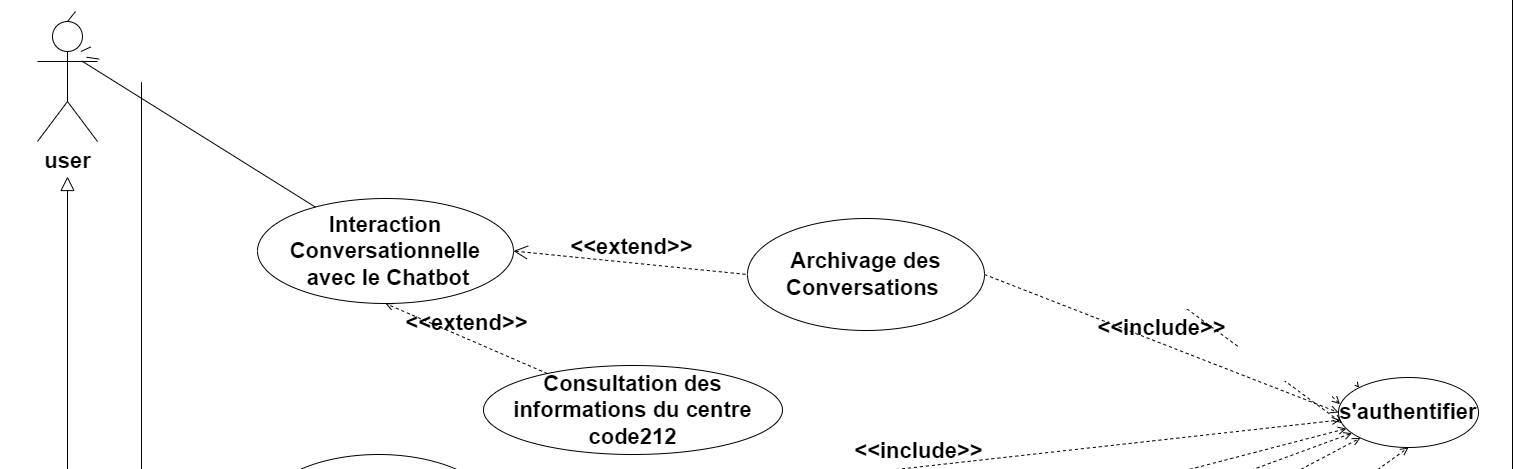
\includegraphics[height=6cm]{assets/images/sprint1-usecase.png}
    \end{figure}
\end{frame}

\begin{frame}{Diagramme de classe}

    \begin{figure}[H]
        \centering
        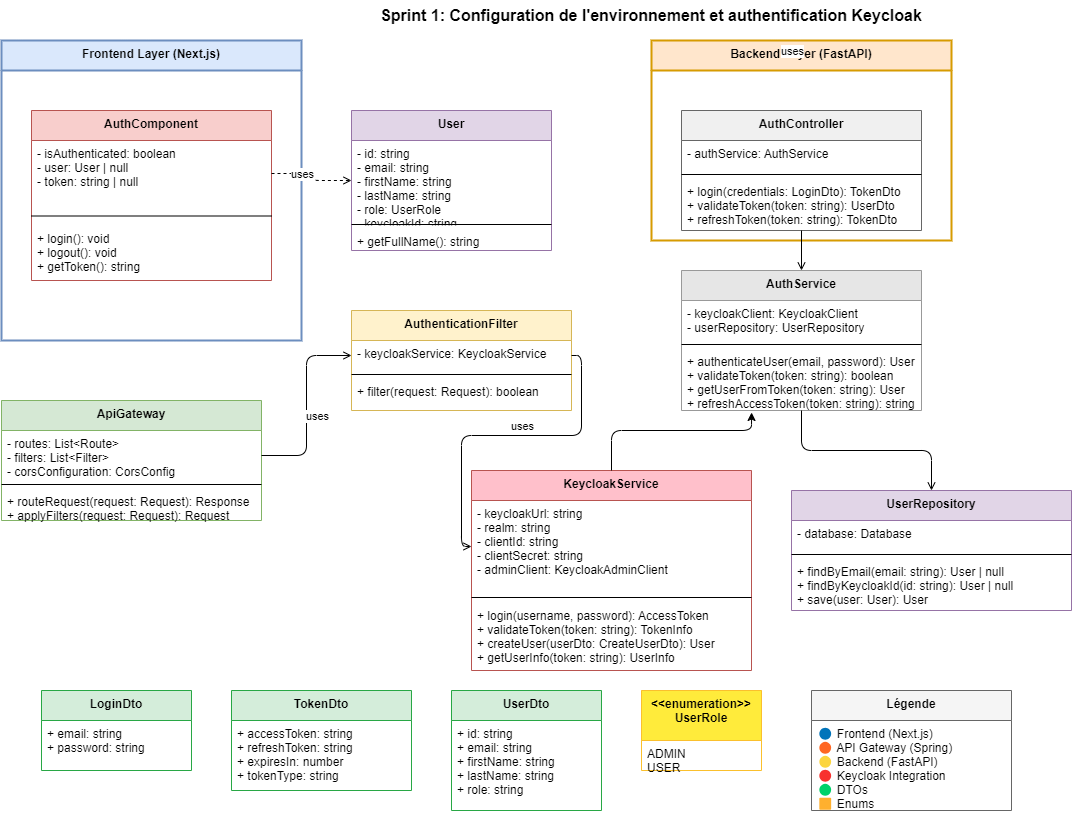
\includegraphics[height=5cm]{assets/images/sprint1-class.png}
    \end{figure}
\end{frame}

\begin{frame}{Diagramme de sequence}
    \begin{figure}[H]
        \centering
        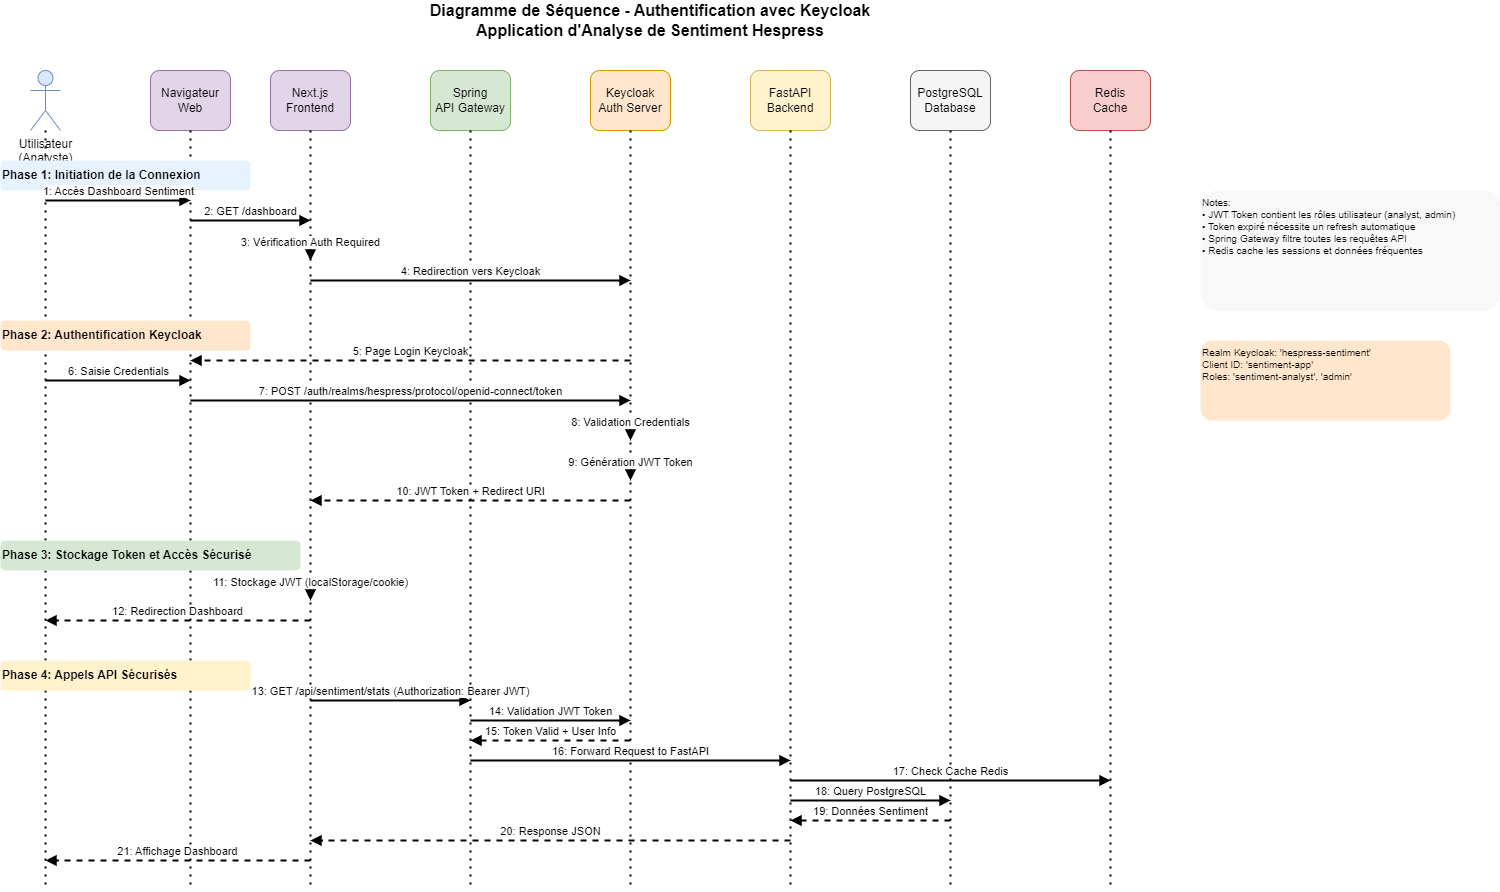
\includegraphics[height=6cm]{assets/images/sprint1-sequence.png}
    \end{figure}
\end{frame}

\begin{frame}{Realisation}
    \begin{figure}[H]
        \centering
        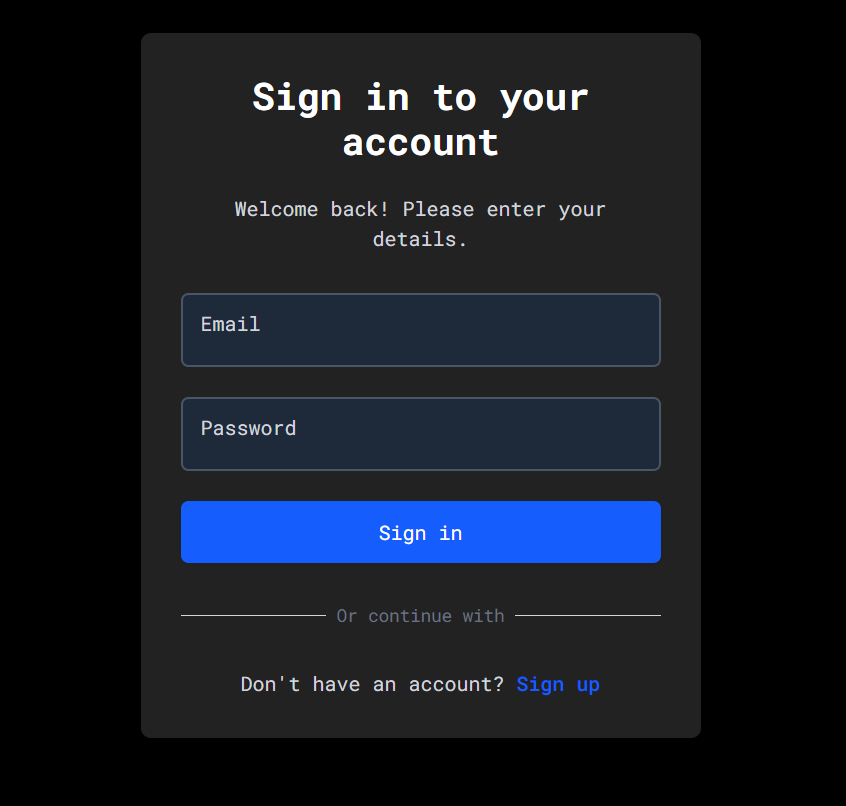
\includegraphics[height=6cm]{assets/images/signin-ui.png}
    \end{figure}
\end{frame}


\subsection{Sprint 2: Développement du module de web scraping et prétraitement des données}
\begin{frame}{Diagramme de cas d'utilisation}

    \begin{figure}[H]
        \centering
        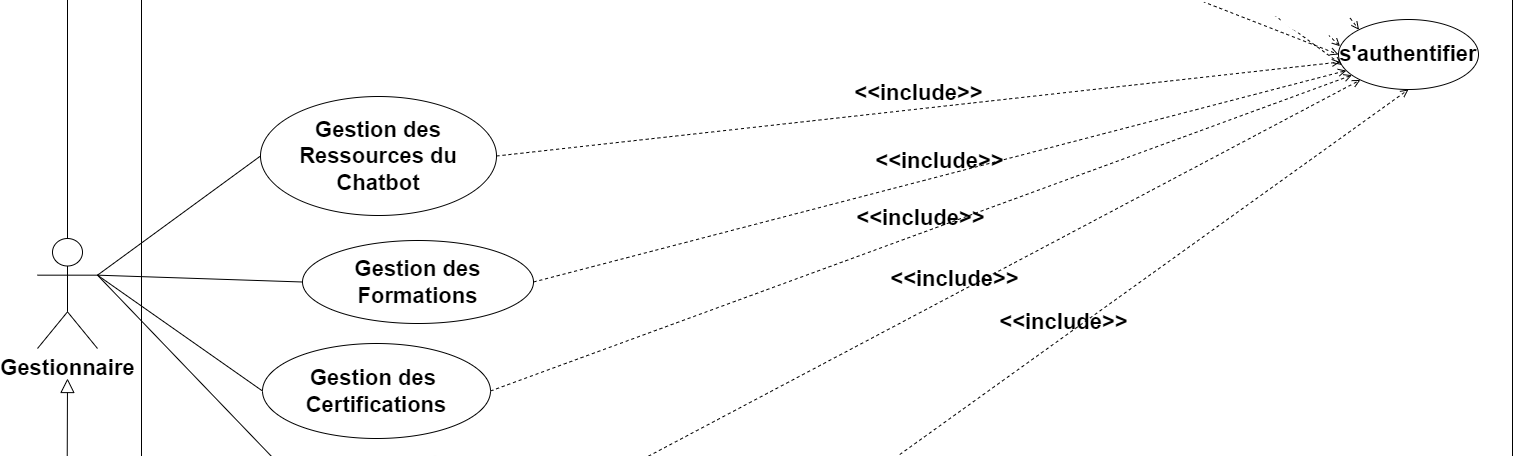
\includegraphics[height=4cm]{assets/images/sprint2-usecase.png}
    \end{figure}
\end{frame}

\begin{frame}{Diagramme de classe}

    \begin{figure}[H]
        \centering
        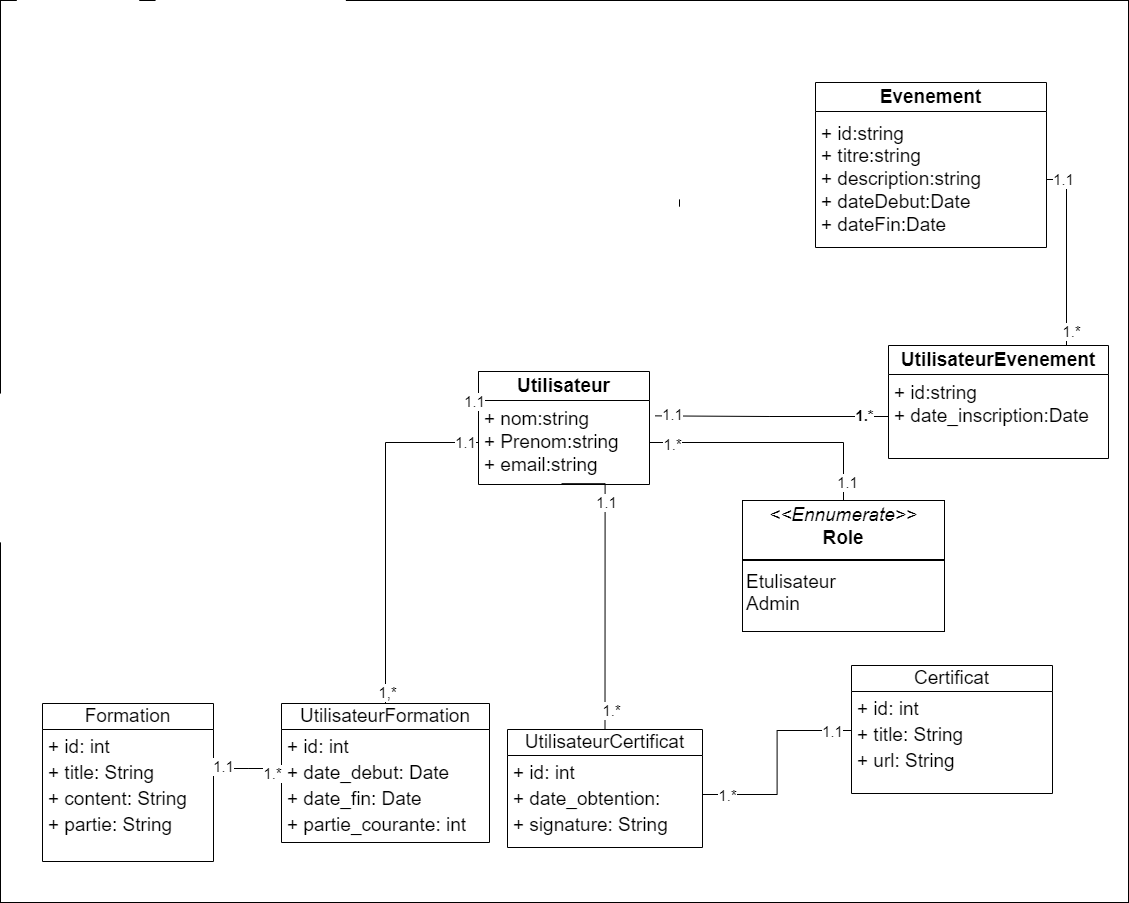
\includegraphics[height=5cm]{assets/images/sprint2-class.png}
    \end{figure}
\end{frame}

\begin{frame}{Diagramme de sequence de récupération des données}
    \begin{figure}[H]
        \centering
        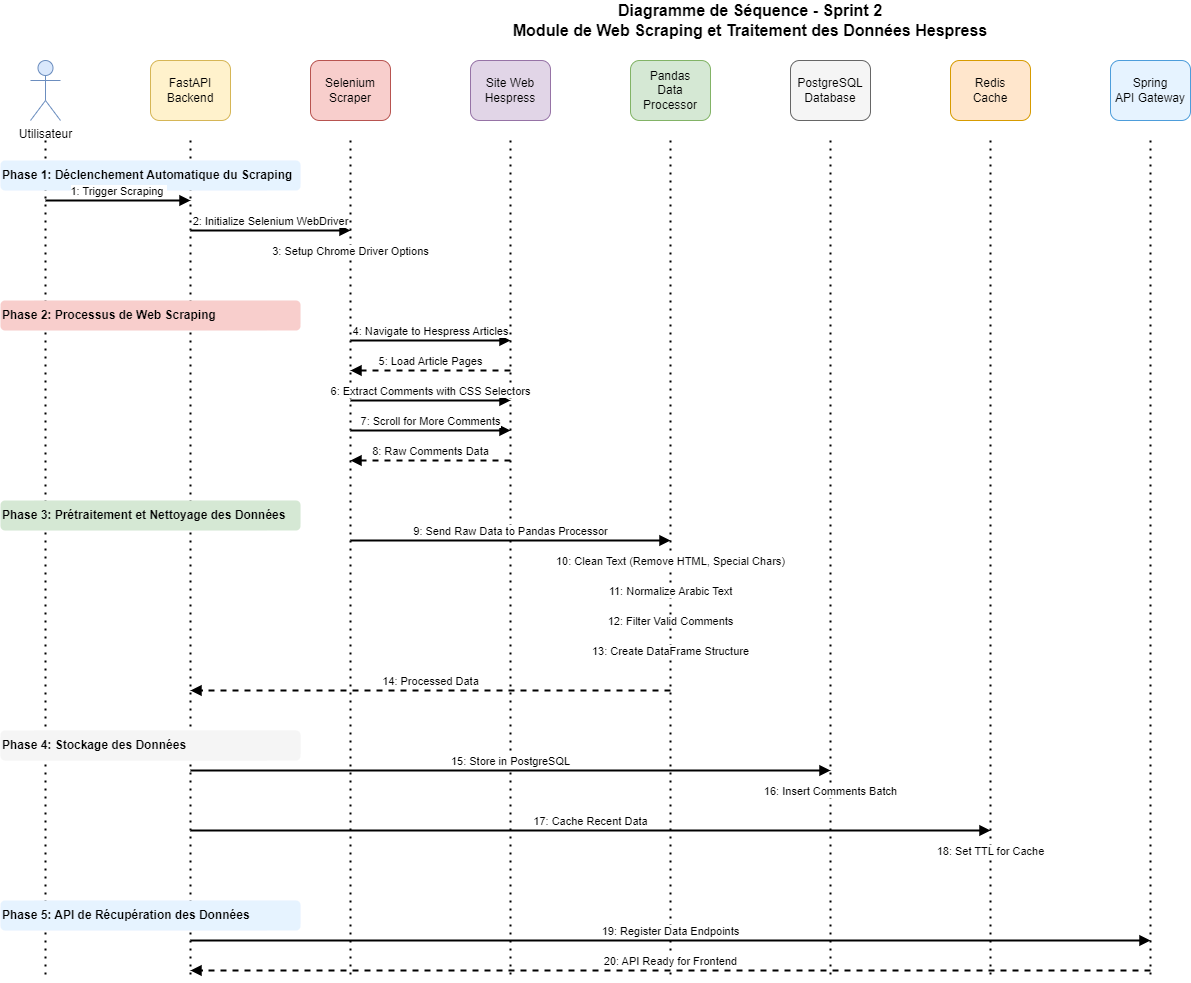
\includegraphics[height=6cm]{assets/images/sprint2-sequence.png}
    \end{figure}
\end{frame}

\begin{frame}{Realisation}
    \begin{figure}[H]
        \centering
        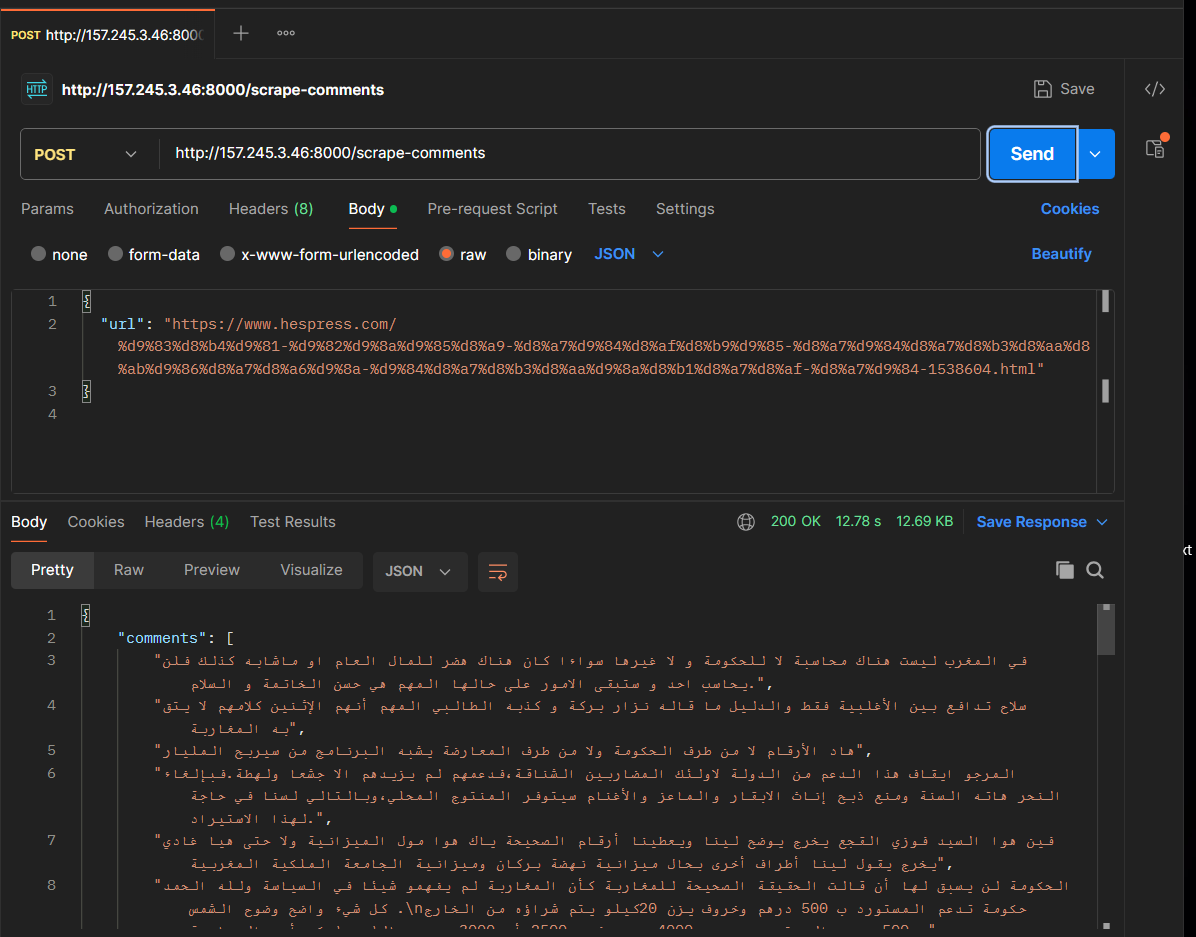
\includegraphics[height=6cm]{assets/images/scrape-ui.png}
    \end{figure}
\end{frame}



\subsection{Sprint 3: Intégration du modèle d'analyse de sentiment et développement du tableau de bord}
\begin{frame}{Diagramme de cas d'utilisation}

    \begin{figure}[H]
        \centering
        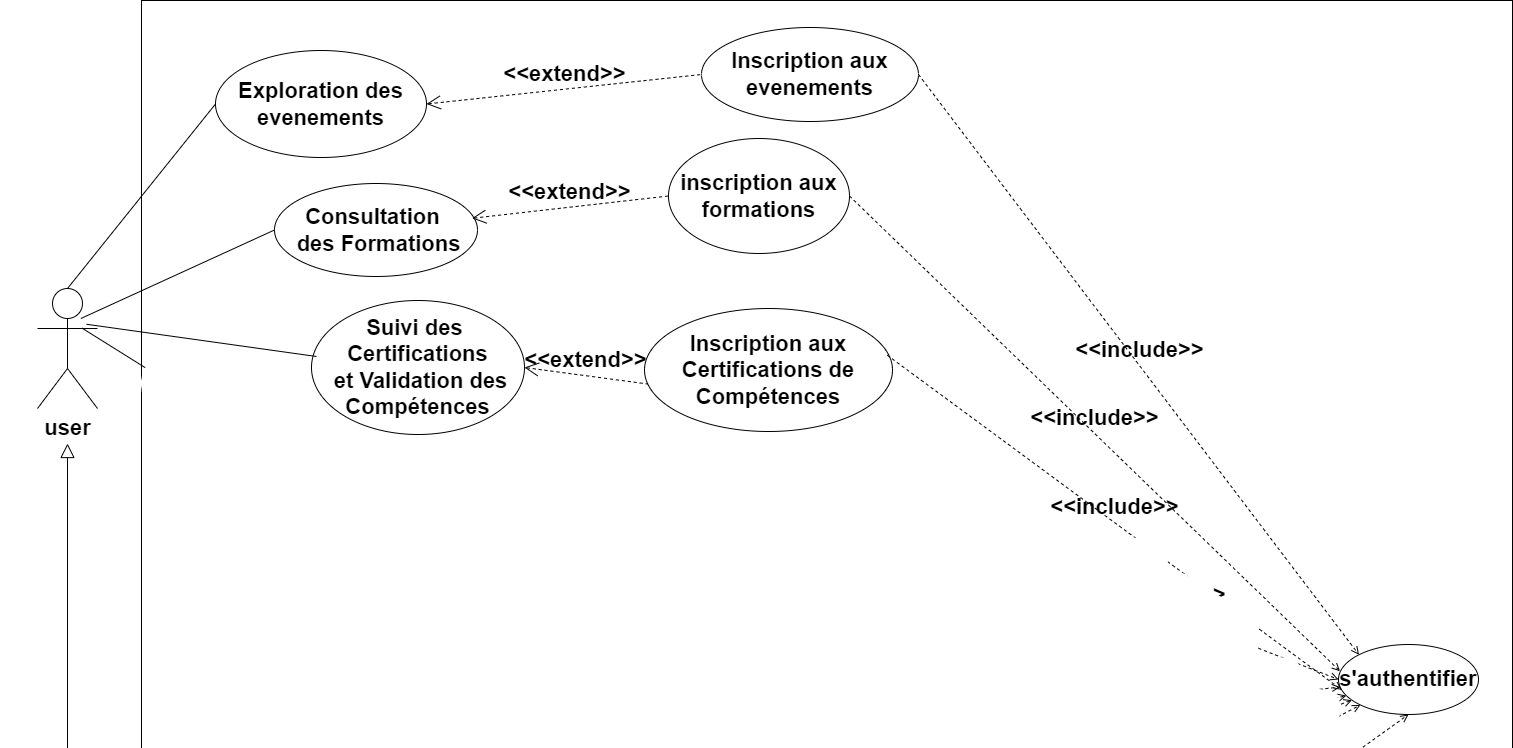
\includegraphics[height=5cm]{assets/images/sprint3-usecase.png}
    \end{figure}
\end{frame}

\begin{frame}{Diagramme de classe}

    \begin{figure}[H]
        \centering
        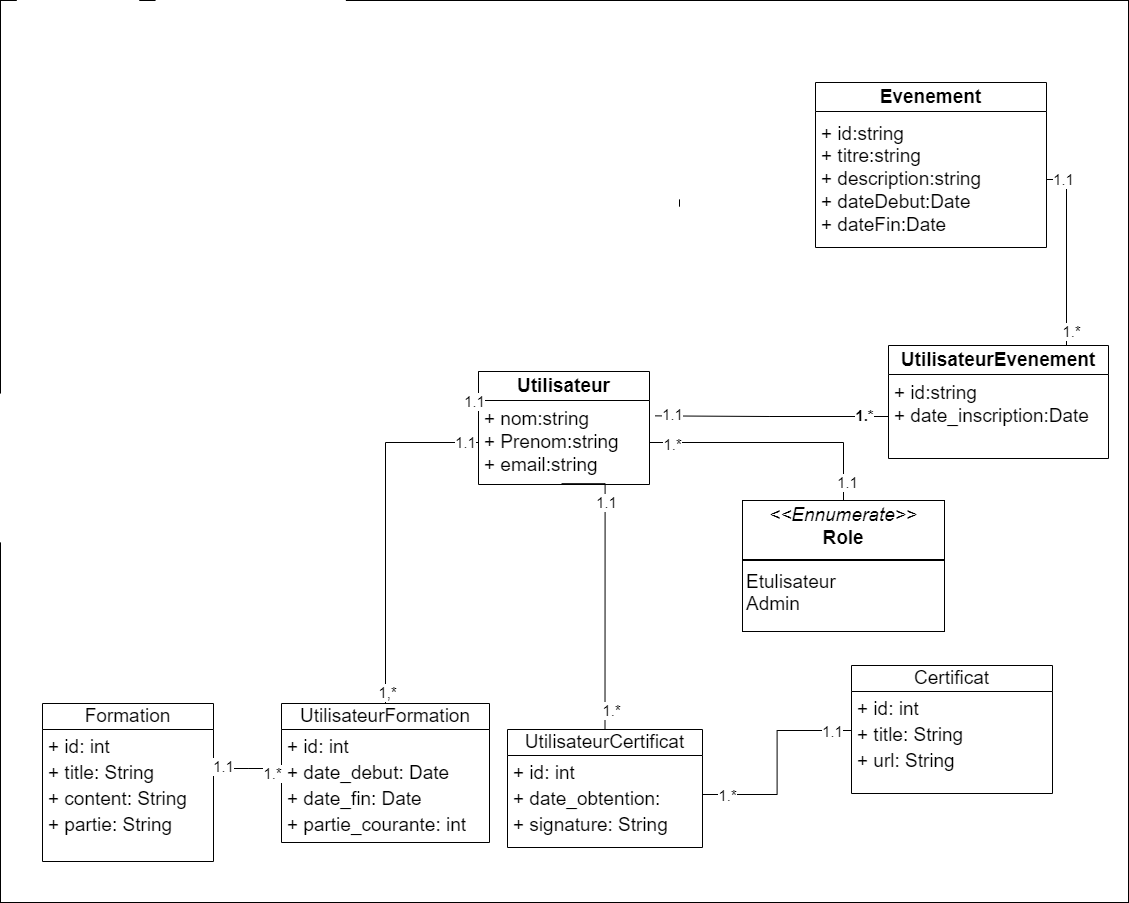
\includegraphics[height=5cm]{assets/images/sprint2-class.png}
    \end{figure}
\end{frame}


\begin{frame}{Diagramme de sequence}
    \begin{figure}[H]
        \centering
        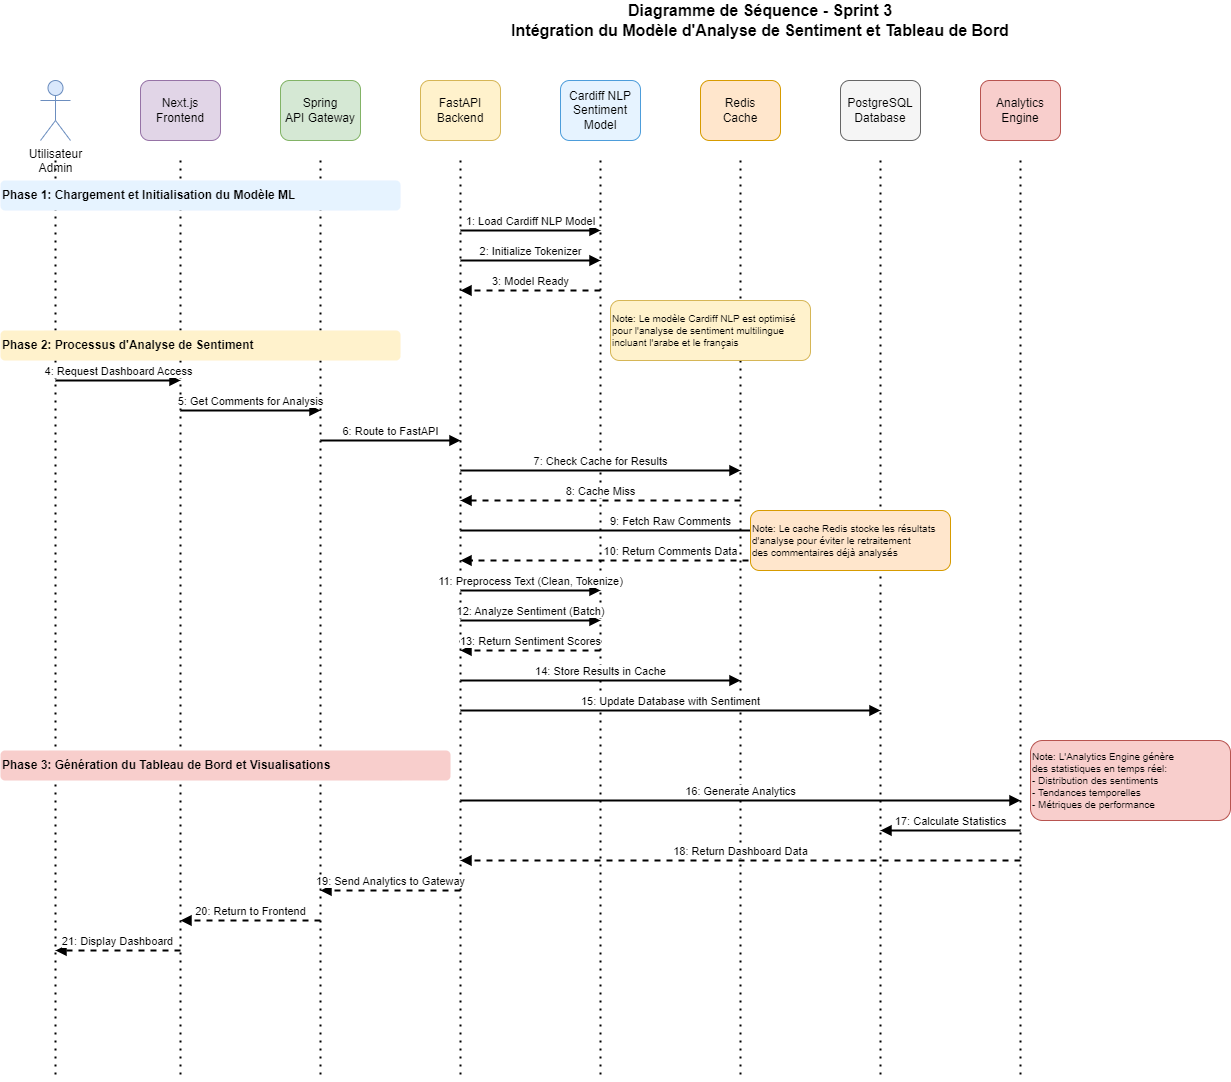
\includegraphics[height=6cm]{assets/images/sprint3-sequence.png}
    \end{figure}
\end{frame}

\begin{frame}{Realisation}
    \begin{figure}[H]
        \centering
        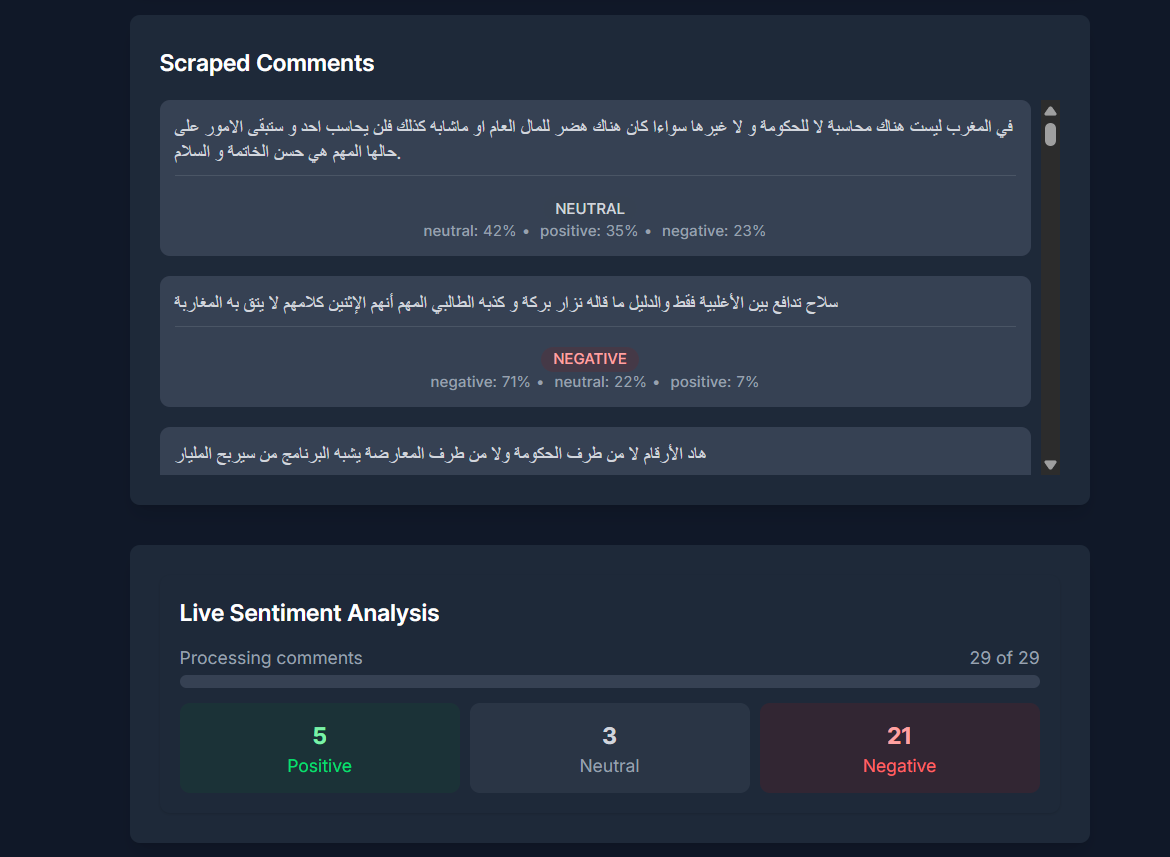
\includegraphics[height=6cm]{assets/images/report-ui.png}
    \end{figure}
\end{frame}




\subsection{Sprint 4: Génération des rapports d'analyse et tests fonctionnels}

\begin{frame}{Interface d'analyse }
    \begin{figure}[H]
        \centering
        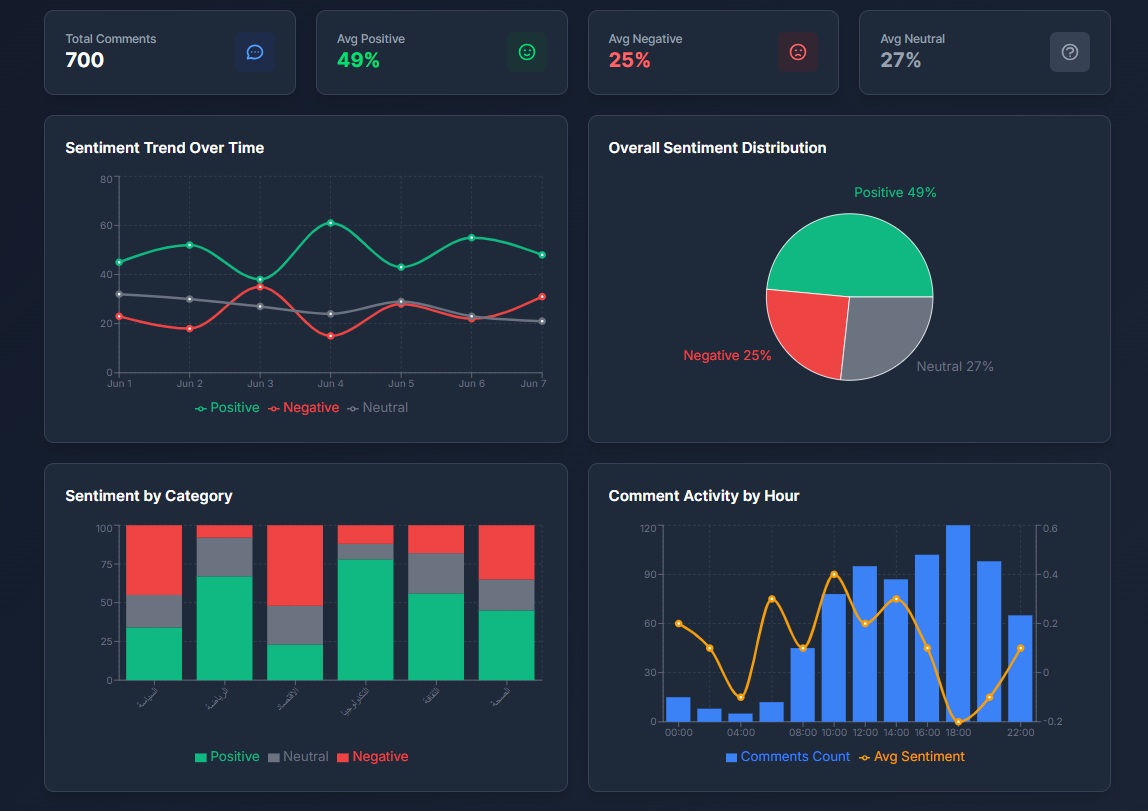
\includegraphics[height=6cm]{assets/images/admin-ui.png}
    \end{figure}
\end{frame}

\begin{frame}{Rapport lighthouse:}
    \begin{figure}[H]
        \centering
        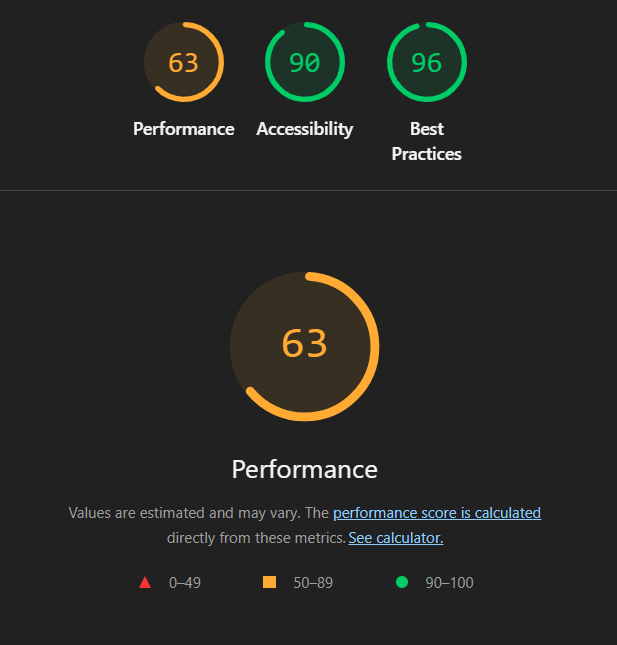
\includegraphics[height=6cm]{assets/images/lighthouse.png}
    \end{figure}
\end{frame}

\subsection{Demmonstration de l'application}
\begin{frame}{Demmonstration de l'application}
    Demonstration de l'application
\end{frame}
